%!TEX root = pset1.tex

\section{Implement Gradient Descent}\label{sec:grad_desc}

\subsection{Implementation}
We implemented a basic gradient descent function in MATLAB. In this function, the user can specify the objective function and the corresponding gradient function. The user also inputs an initial guess, the constant step size, and the convergence threshold.  The algorithm works as follows: starting at the initial guess, we move to a new point by taking a step (of the specified step size) in the direction of the gradient. We repeat the process until the difference in objective value between two subsequent iterations is less than the specified threshold.

\subsection{Testing Gradient Descent}
We test the gradient descent method on the following functions:
\begin{enumerate}
\item $f(x_1, x_2) = 3x_1^2 + 2x_1x_2 + x_2^2 - 4x_1 + 5x_2$ \\
	By completing the square we find that the optimal solution is: $x_1 = 2.25, x_2 = -4.75$, and the optimal value is: $f(x_1, x_2) = -16.375$.
\item $f(x) = -\frac{1}{\sqrt{2\pi}\sigma}e^{-(x-\mu)^2/2\sigma^2}$ \\
	This is the negative of a Gaussian pdf, with $\mu = 0$ and $\sigma = 1$.  The optimal solution is $x = 0$ and the optimal value is: $f(x) = -\frac{1}{\sqrt{2\pi}}$.
\item $f(x) = x^3 - 10x$.\\
	This is not a convex function.  There is one local minimum: $x = 1.8257$, $f(x) = -12.17$, but the global minimum is negative infinity.
\end{enumerate}

The basic gradient descent method works well on the first two functions. For most specifications of the initial guess and step size, the procedure converges to the right answer. Increasing the convergence threshold to very large values leads to imprecise results, and decreasing it to very small values results in more iterations until convergence. In some cases, very large or very small step sizes may result in non-convergence. For the third function which is non-convex, selecting an initial guess $x_0 \geq -1.8257$ leads us to the incorrect, local minimum.  

\begin{figure}[h!]
\centering
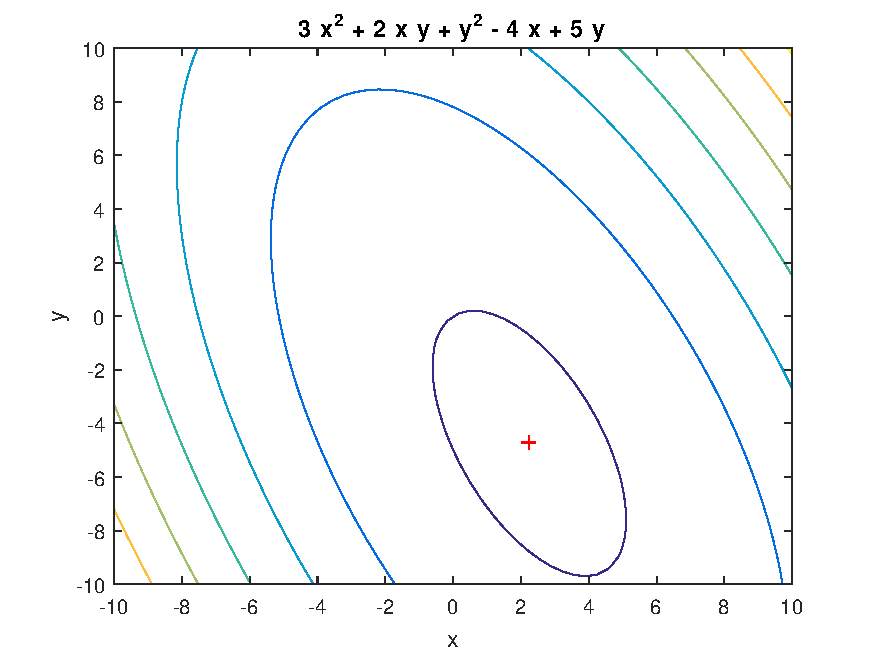
\includegraphics[scale=0.4]{hw1_1.pdf}
\caption{Contour plot of the first function. The gradient descent method moves in steps (blue dots) towards the local/global optimum (red cross).}
\end{figure}


\subsection{Numerical Gradient}
We can also numerically evaluate the gradient at a given point. The partial derivative at $x_i$ is approximated by the formula below, where $\V h$ is the vector of all zeros except for the $i$th component that is $\epsilon$.  We apply this numerical gradient in place of the analytic one in the original three functions.  For sufficiently small $\epsilon$, the results are almost identical.
%
\begin{equation}
\frac{\partial f(\V x)}{\partial x_i} = \frac{f(\V x+\V h) - f(\V x-\V h)}{2\epsilon}
\end{equation}

\subsection{Comparing with Sophisticated Methods}
As the final step to evaluate our implementation of gradient descent, we compare our method against state-of-the-art gradient descent packages in MATLAB.  Compared against \texttt{fminunc}, our implementation is dramatically slower. For example, given the same convergence criterion, it takes 35 iterations for our method to converge, while \texttt{fminunc} converges after 8 iterations.  We think the disadvantage is due to the constant step size in our method. Since the step size does not adapt while the algorithm is running, our method is likely to undershoot or overshoot the optimal solution. An improvement could be made using backtracking, exact line-search, or other techniques to adaptively update the step size.  